\newif\ifshowsolutions
\showsolutionstrue
\documentclass{article}
\usepackage{listings}
\usepackage{amsmath}
%\usepackage{subfigure}
\usepackage{subfig}
\usepackage{amsthm}
\usepackage{amsmath}
\usepackage{amssymb}
\usepackage{graphicx}
\usepackage{mdwlist}
\usepackage[colorlinks=true]{hyperref}
\usepackage{geometry}
\usepackage{titlesec}
\geometry{margin=1in}
\geometry{headheight=2in}
\geometry{top=2in}
\usepackage{palatino}
\usepackage{mathrsfs}
\usepackage{fancyhdr}
\usepackage{paralist}
\usepackage{todonotes}
\setlength{\marginparwidth}{2.15cm}
\usepackage{tikz}
\usetikzlibrary{positioning,shapes,backgrounds}
\usepackage{float} % Place figures where you ACTUALLY want it
\usepackage{comment} % a hack to toggle sections
\usepackage{ifthen}
\usepackage{mdframed}
\usepackage{verbatim}
\usepackage[strings]{underscore}
\usepackage{listings}
\usepackage{bbm}
\rhead{}
\lhead{}

\renewcommand{\baselinestretch}{1.15}

% Shortcuts for commonly used operators
\newcommand{\E}{\mathbb{E}}
\newcommand{\Var}{\operatorname{Var}}
\newcommand{\Cov}{\operatorname{Cov}}
\newcommand{\Bias}{\operatorname{Bias}}
\DeclareMathOperator{\argmin}{arg\,min}
\DeclareMathOperator{\argmax}{arg\,max}

% do not number subsection and below
\setcounter{secnumdepth}{1}

% custom format subsection
\titleformat*{\subsection}{\large\bfseries}

% set up the \question shortcut
\newcounter{question}[section]
\newenvironment{question}[1][]
  {\refstepcounter{question}\par\addvspace{1em}\textbf{Question~\Alph{question}\!
    \ifthenelse{\equal{#1}{}}{}{ [#1 points]}: }}
    {\par\vspace{\baselineskip}}

\newcounter{subquestion}[question]
\newenvironment{subquestion}[1][]
  {\refstepcounter{subquestion}\par\medskip\textbf{\roman{subquestion}.\!
    \ifthenelse{\equal{#1}{}}{}{ [#1 points]:}} }
  {\par\addvspace{\baselineskip}}

\titlespacing\section{0pt}{12pt plus 2pt minus 2pt}{0pt plus 2pt minus 2pt}
\titlespacing\subsection{0pt}{12pt plus 4pt minus 2pt}{0pt plus 2pt minus 2pt}
\titlespacing\subsubsection{0pt}{12pt plus 4pt minus 2pt}{0pt plus 2pt minus 2pt}


\newenvironment{hint}[1][]
  {\begin{em}\textbf{Hint: }}{\end{em}}

\ifshowsolutions
  \newenvironment{solution}[1][]
    {\par\medskip \begin{mdframed}\textbf{Solution~\Alph{question}#1:} \begin{em}}
    {\end{em}\medskip\end{mdframed}\medskip}
  \newenvironment{subsolution}[1][]
    {\par\medskip \begin{mdframed}\textbf{Solution~\Alph{question}#1.\roman{subquestion}:} \begin{em}}
    {\end{em}\medskip\end{mdframed}\medskip}
\else
  \excludecomment{solution}
  \excludecomment{subsolution}
\fi



%%%%%%%%%%%%%%%%%%%%%%%%%%%%%%
% HEADER
%%%%%%%%%%%%%%%%%%%%%%%%%%%%%%

\chead{
  {\vbox{
      \vspace{2mm}
      \large
      Machine Learning \& Data Mining \hfill
      Caltech CS/CNS/EE 155 \hfill \\[1pt]
      Set 3\hfill
      January $26^\text{th}$, 2022 \\
    }
  }
}

\begin{document}
\pagestyle{fancy}



%%%%%%%%%%%%%%%%%%%%%%%%%%%%%%
% POLICIES
%%%%%%%%%%%%%%%%%%%%%%%%%%%%%%

\section*{Policies}
\begin{itemize}
	\item Due 9 PM PST, January $26^\text{th}$ on Gradescope. 
	\item You are free to collaborate on all of the problems, subject to the collaboration policy stated in the syllabus.
	\item In this course, we will be using Google Colab for code submissions. You will need a Google account.
\end{itemize}

\section*{Submission Instructions}
\begin{itemize}
	\item Submit your report as a single .pdf file to Gradescope, under "Set 3 Report". 
	\item In the report, \textbf{include any images generated by your code} along with your answers to the questions.
	\item Submit your code by \textbf{sharing a link in your report} to your Google Colab notebook for each problem (see naming instructions below). Make sure to set sharing permissions to at least "Anyone with the link can view". \textbf{Links that can not be run by TAs will not be counted as turned in.} Check your links in an incognito window before submitting to be sure. 
	\item For instructions specifically pertaining to the Gradescope submission process, see \url{https://www.gradescope.com/get_started#student-submission}.
\end{itemize}

\section*{Google Colab Instructions}
For each notebook, you need to save a copy to your drive.
\begin{enumerate}
	\item Open the github preview of the notebook, and click the icon to open the colab preview.
	\item On the colab preview, go to File $\rightarrow$ Save a copy in Drive.
	\item Edit your file name to “lastname_firstname_set_problem”, e.g.”yue_yisong_set3_prob2.ipynb”
\end{enumerate}

%%%%%%%%%%%%%%%%%%%%%%%%%%%%%%
% PROBLEM 1
%%%%%%%%%%%%%%%%%%%%%%%%%%%%%%

\newpage
\section{Decision Trees [30 Points]}
\materials{Lecture 5}

\problem[7]
Consider the following data, where given information about some food you must predict whether it is healthy:

\begin{table}[ht]
\centering
\begin{tabular}{c | c c c | c}
\hline
No. & Package Type & Unit Price $>$ \$5 & Contains $>$ 5 grams of fat & Healthy? \\ [0.5ex]
\hline
1 & Canned & Yes & Yes & No  \\
2 & Bagged & Yes & No  & Yes \\
3 & Bagged & No  & Yes & Yes \\
4 & Canned & No  & No  & Yes \\ [1ex]
\hline
\end{tabular}
\end{table}

Train a decision tree by hand using top-down greedy induction. Use \emph{entropy} (with natural log) as the impurity measure.  Since the data can be classified
without error, the stopping criterion will be no impurity in the leaves.

Submit a drawing of your tree showing the impurity reduction yielded by each split (including root) in your decision tree.

\begin{solution}
 Starting at the root node, we have $|S|=4$ and $p_S = 0.75$, thus the entropy is 2.25.

 At the first node, we find that all three splits have the same entropy:
 \begin{itemize}
     \item Package type: Canned = \{no,yes\}, Bagged = \{yes,yes\}; entropy = 1.38
     \item Unit Price > \$5: Yes = \{no,yes\}, No = \{yes,yes\}; entropy = 1.38
     \item Contains > 5 grams of fat: Yes = \{no,yes\}, No = \{yes,yes\}; entropy = 1.38
 \end{itemize}
 As such, there is no difference between which split we choose. Randomly selecting package type, we get, for canned:
 \begin{itemize}
     \item Unit price > \$5: Yes = \{no\}, No = \{yes\}; entropy = 0.00
     \item Contains > 5 grams of fat: Yes = \{no\}, No = \{yes\}; entropy = 0.00
 \end{itemize}
 Again, both entropies are identical and give us an impurity of 0.00, as such, by picking either of the above, we have reached our stopping criteria, giving the following tree with their respective reductions:
 \begin{figure}[H]
    \begin{center}
    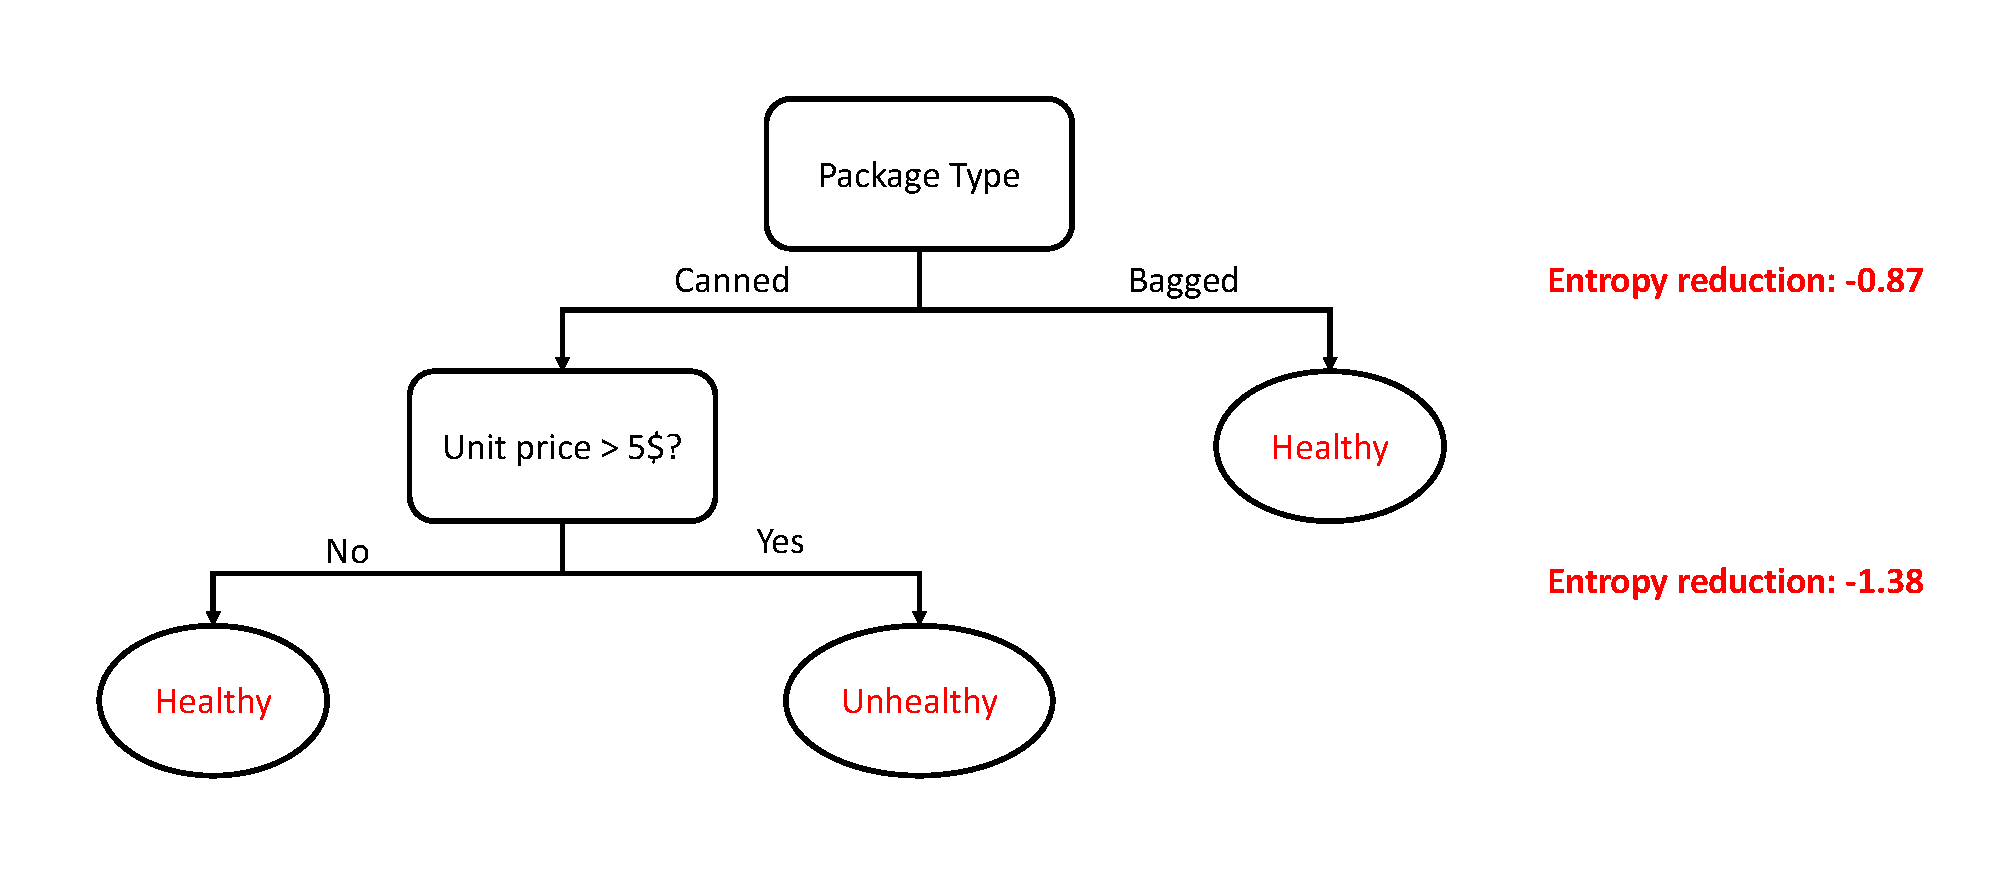
\includegraphics[width=\textwidth]{Tree_1A.pdf}
    \end{center}
    \end{figure}
\end{solution}

\problem[4]
Compared to a linear classifier, is a decision tree always preferred for classification problems? If not, draw a simple 2-D dataset that can be perfectly classified by a simple linear classifier but which requires an overly complex decision tree to perfectly classify.

\begin{solution}
  The tree classifier model is not always preferrable to the linear classifier. An example of this is shown below:
  \begin{figure}[H]
    \begin{center}
    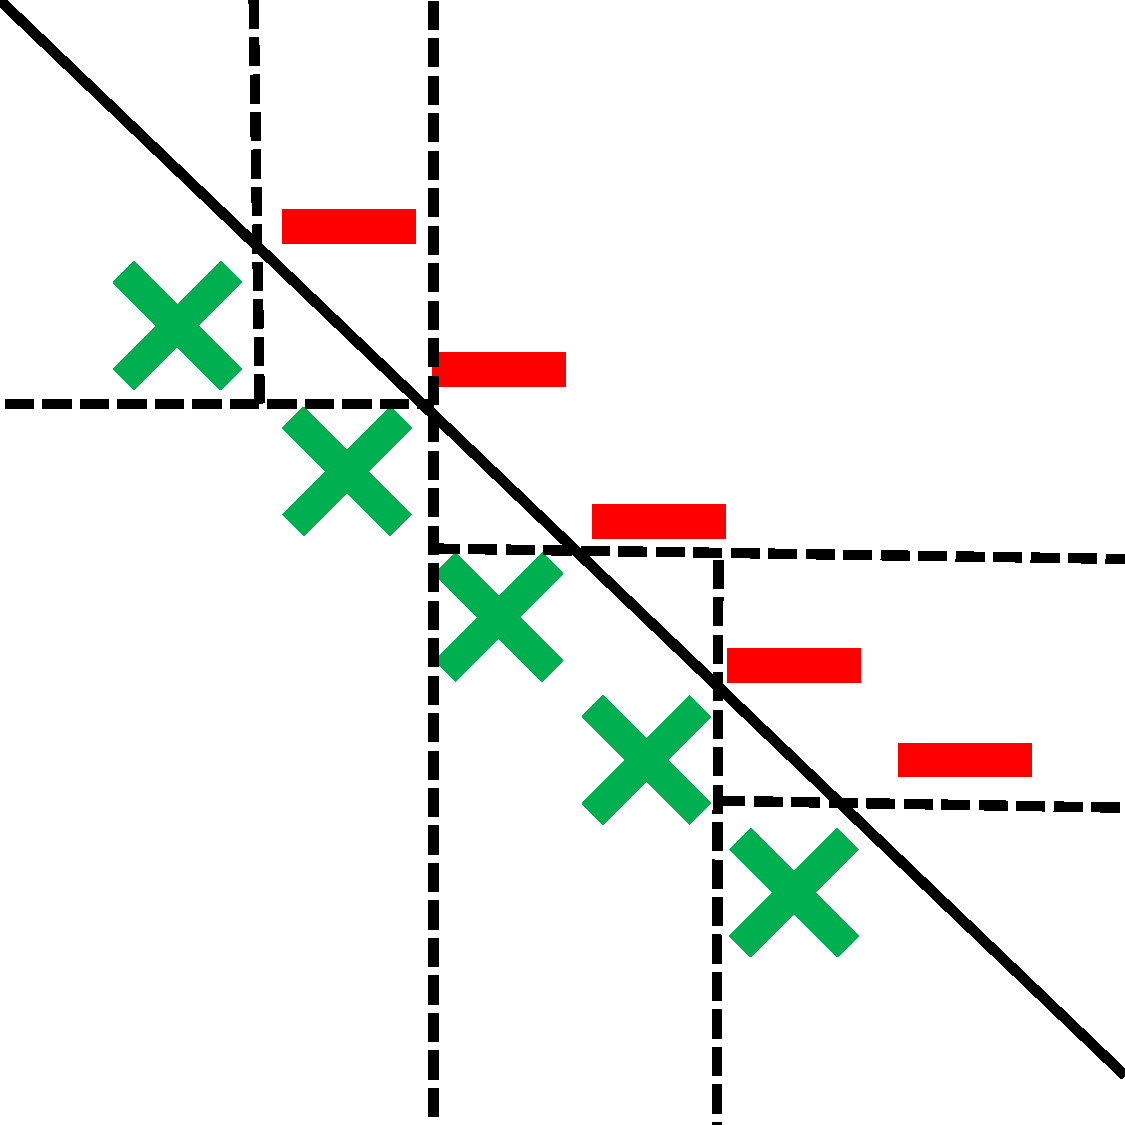
\includegraphics[width=0.7\textwidth]{LinSepSet.pdf}
    \end{center}
    \end{figure}
    As we can see above, there are many wasted boundaries.
\end{solution}

\problem[15]
Consider the following 2D data set:
\begin{figure}[H]
    \begin{center}
    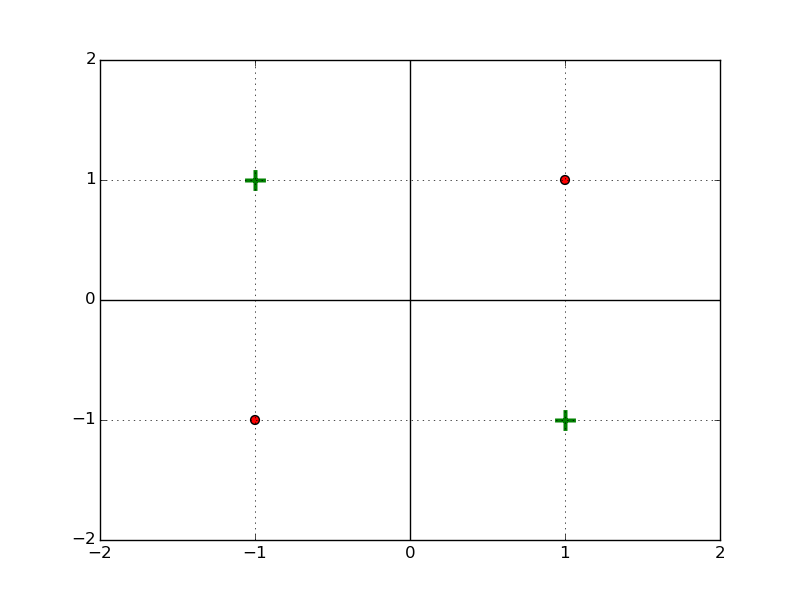
\includegraphics[width=3.3in]{plots/3C.png}
    \end{center}
    \end{figure}

\subproblem[5] Suppose we train a decision tree on this dataset using top-down greedy induction, with the Gini index as
the impurity measure. We define our stopping condition to be if no split of a node
results in any reduction in impurity. Submit a drawing of the resulting tree.  What is its classification error ((number of misclassified points) / (number of total points))?

\subproblem[5] Submit a drawing of a two-level decision tree that classifies the above dataset with zero classification error.  (You don't need to use any particular training algorithm to produce the tree.)

Is there any impurity measure (i.e. any function that maps the data points under a particular node in a tree to a real number) that would have led top-down greedy induction with the same stopping condition to produce the tree you drew?  If so, give an example of one, and briefly describe its pros and cons as an impurity measure for training decision trees in general (on arbitrary datasets). 

\subproblem[5] Suppose there are 100 data points in some 2-D dataset. What is the largest number of unique thresholds (i.e., internal nodes) you might need in order to achieve zero classification training error (on the training set)? Please
justify your answer.

\begin{solution}
    \begin{itemize}
        \item Trying to split this data set, we find that all linear, single-level splits will result in the same impurity of 2.0. As such, the classification error will be (2/4)=0.5. The true is simply: 
        \begin{figure}[H]
           \begin{center}
           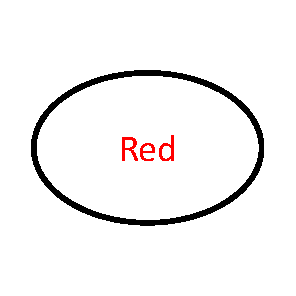
\includegraphics[width=0.3\textwidth]{Tree_1Ci.pdf}
           \end{center}
           \end{figure}
        \item The following tree will result in a classification error of 0:
        \begin{figure}[H]
            \begin{center}
            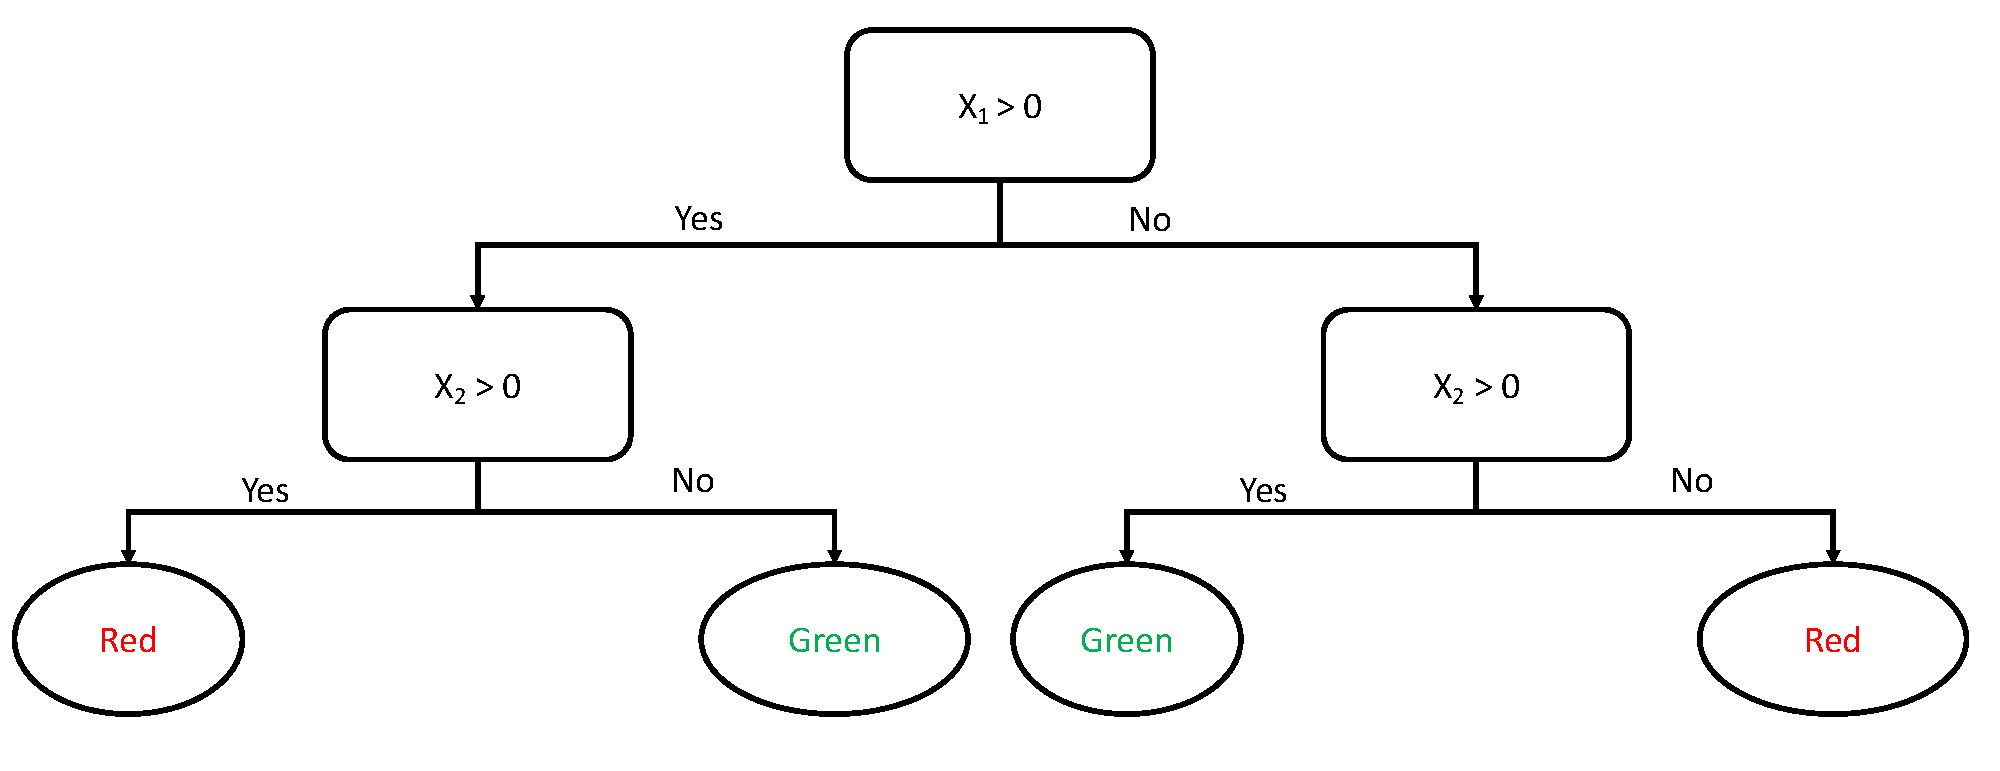
\includegraphics[width=0.7\textwidth]{Tree_1Cii.pdf}
            \end{center}
            \end{figure}
        The following impurity measure would lead to a top-down greedy induction with the same stopping conduction to produce the above tree:
        \begin{equation}
            \text{impurity} = \frac{\#\text{pos}\times\#\text{neg}}{\sqrt{|S'|}}
        \end{equation}
        Pros: This effectively ensures that, if the fraction of correct classifications is the same before and after the split, we will split. 

        Cons: This preference towards splitting may lead to unnecessary splits which can lead to overfitting. For example, in the case where the fraction of correct classifications is the same before and after the split, this split may actually result in worse generalisability of the tree.

        \item If we imagine a case where the points are alternating between classifiers along both of the axis, the number of splits required to give a 0 training error will be however many data points - 1; this is the worst-case scenario for classifying a data set. As such, for a data set of 100 points, the maximum number of splits required with be 99 splits.
    \end{itemize}
 
\end{solution}

\problem[4] Suppose in top-down greedy induction we want to split a leaf node that contains N data points composed of
D continuous features. What is the worst-case
complexity (big-O in terms of N and D) of the number of possible splits we must consider in order to find the one that most reduces impurity? Please justify your answer.

Note: Recall that at each node-splitting step in training a DT, you must consider all possible splits that you can make. While there are an infinite number of possible decision boundaries since we are using continuous features, there are not an infinite number of boundaries that result in unique child sets (which is what we mean by ``split'').

\begin{solution}
   In the worst-case complexity scenario, where the data set can only be split into the specific coordinates (or `cells') of the data points, we will need $\mathcal{O}(ND)$ splits. The best way to illustrate this is, like in the 2D example above, if the data points are alternating in all dimensions D, we will need $\mathcal{O}(ND)$ splits. 
\end{solution}


\newpage


\section{Overfitting Decision Trees [30 Points, EC 7 Points]}
\materials{Lecture 5}

In this problem, you will use the Diabetic Retinopathy Debrecen Data Set, which contains features extracted from images to determine whether or not the images contain signs of diabetic retinopathy. Additional information about this dataset can be found at the link below:

\url{https://archive.ics.uci.edu/ml/datasets/Diabetic+Retinopathy+Debrecen+Data+Set}

In the following question, your goal is to predict the diagnosis of diabetic retinopathy, which is the final column in the data matrix.  Use the first 900 rows as training data, and the last
251 rows as validation data. Please feel free to use additional packages such as Scikit-Learn. Include your code in your submission.


\indent\problem[10] \smallskip 
Choose one of the following from i or ii: 

\noindent i. Train a decision tree classifier using Gini as the impurity measure and minimal leaf node size as early stopping criterion. Try different minimal leaf node sizes from 1 to 25 in increments of 1. Then, on a single plot, plot both training and test classification error versus leaf node size. To do this, fill in the \texttt{classification_err} and \texttt{eval_tree_based_model_min_samples} functions in the code template for this problem.


ii. Train a decision tree classifier using Gini as the impurity measure and maximal tree depth as early stopping criterion. Try different tree depths from 2 to 20 in increments of 1. Then, on a single plot, plot both training and test classification error versus tree depth. To do this, fill in the \texttt{eval_tree_based_model_max_depth} function in the code template for this problem.

\begin{solution}
 
     i. The following figure was generated:
     \begin{figure}[H]
        \begin{center}
        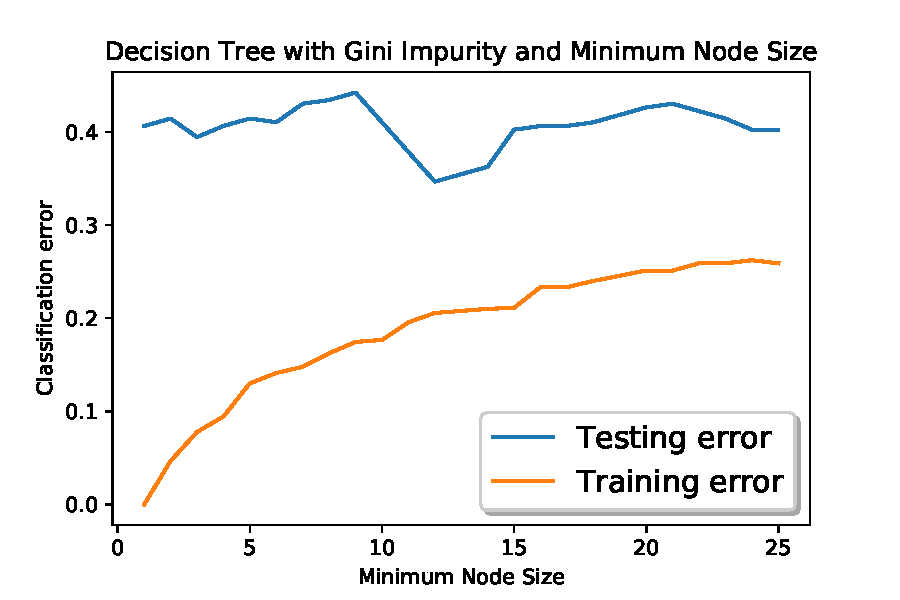
\includegraphics[width=0.7\textwidth]{DT_min_leaf.pdf}
        \end{center}
        \end{figure}
 
\end{solution}

\problem[6]
For either the minimal leaf node size or maximum depth parameters in the previous problem, which parameter value minimizes the test error? What effects does early stopping have on the performance of a decision tree model?
Please justify your answer based on the plot you derived.

\begin{solution}
   In this case, the test error is minimised at a minimum node size of 12. We will have early stopping here at larger minimum node sizes; as such, in decreasing the minimum node size, we will begin to observe overfitting. This is illustrated in the figure with the increasing bias between the testing and training error. Once we introduce early stopping at greater minimum nodes sizes, where we have less splitting, the bias decreases, implying our model will generalise better.
\end{solution}

\indent\problem[4] Choose one of the following from i or ii: \smallskip 

\noindent i. Train a random forest classifier using Gini as the impurity measure, minimal leaf node size as early stopping criterion, and 1,000 trees in the forest. Try different node sizes from 1 to 25 in increments of 1. Then, on a single plot, plot both training and test classification error versus
leaf node size.

ii. Train a random forest classifier using Gini as the impurity measure, maximal tree depth as early stopping criterion, and 1,000 trees in the forest. Try different tree depths from 2 to 20 in increments of 1. Then, on a single plot, plot both training and test classification error versus tree depth.

\begin{solution}
    i. The following figure was generated:
    \begin{figure}[H]
        \begin{center}
        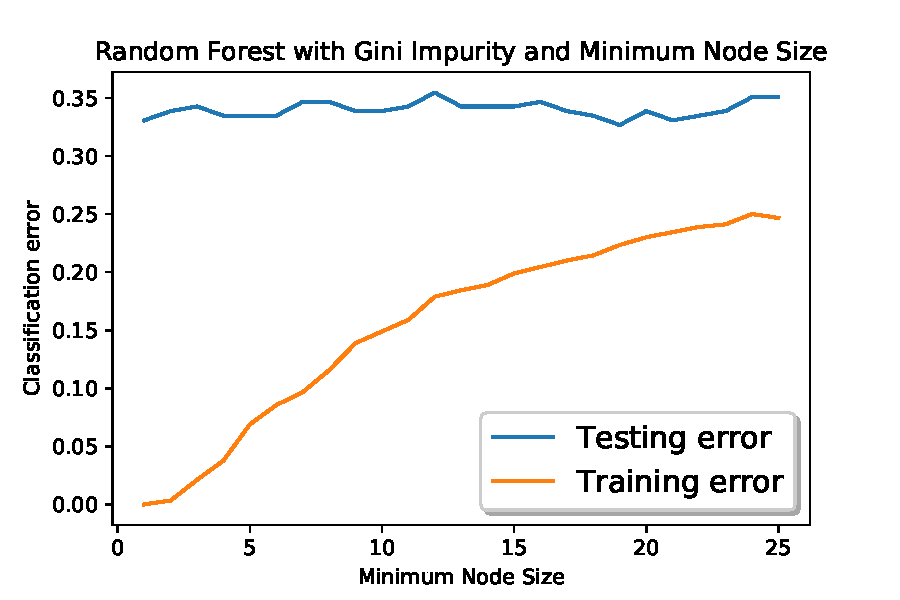
\includegraphics[width=0.7\textwidth]{RT_min_leaf.pdf}
        \end{center}
        \end{figure}
\end{solution}

\problem[6]
For either the minimal leaf node size or maximum depth parameters tested, which parameter value minimizes the random forest test error? What effects does early stopping have on the performance of a random forest model?
Please justify your answer based on the plot you derived.

\begin{solution}
 For minimal leaf node size, we find that a value of 19 minimises the test error. In contrast to the decision tree, the random forest isn't as significantly affected by the early stopping (here indicated by the larger minimal leaf node size). However, like the decision tree, there is overfitting occuring at smaller minimum node size as illustrated by the larger bias. Similarly, with earlier stopping, the bias is reduced, implying the model will generalise better.
\end{solution}

\problem[4]
Do you observe any differences between the curves for the random forest and decision tree plots? If so, explain what could account for these differences.

\begin{solution}
 The impact of the minimal leaf node size is less pronounced in the case of the random forest plot, where our minimum test error is as significantly different compared to the rest of the plot. The magnitude of the testing error is also smaller in the case of the random forest, despite the training error being very similar between the two.

 The reason for this can be accounted for by the fact that the random forest is an ensemble of decision trees where we have generated bootstraps from the original training set and average the results. This will reduce variance in our predictions, as shown above.
\end{solution}

\textbf{Extra Credit [7 points total] :} \problem\textbf{[5 points, Extra Credit]} Complete the other option for \textbf{Problem A }and \textbf{Problem C}.

\begin{solution}
    \begin{figure}[H]
        \subfloat[]{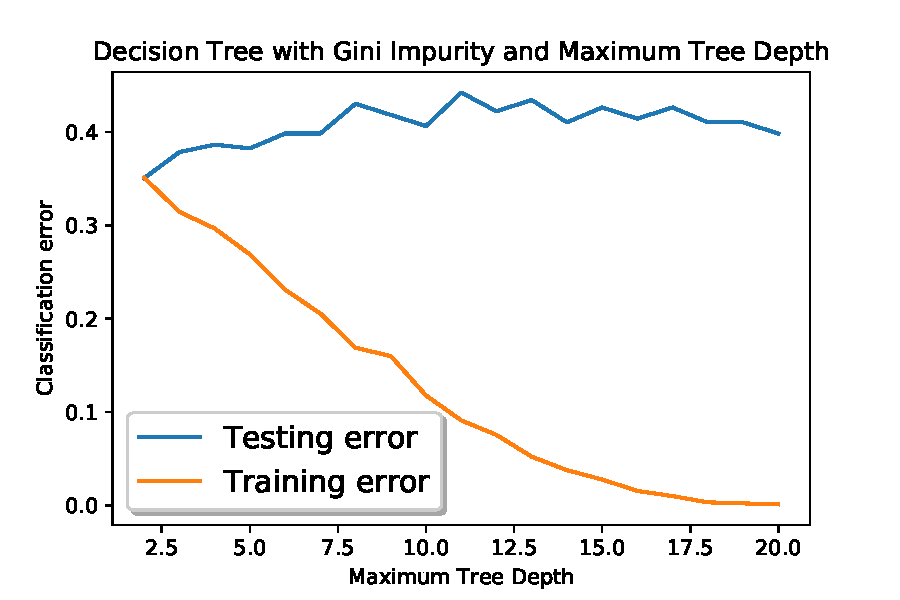
\includegraphics[width=0.49\textwidth]{DT_max_depth.pdf}}
        \subfloat[]{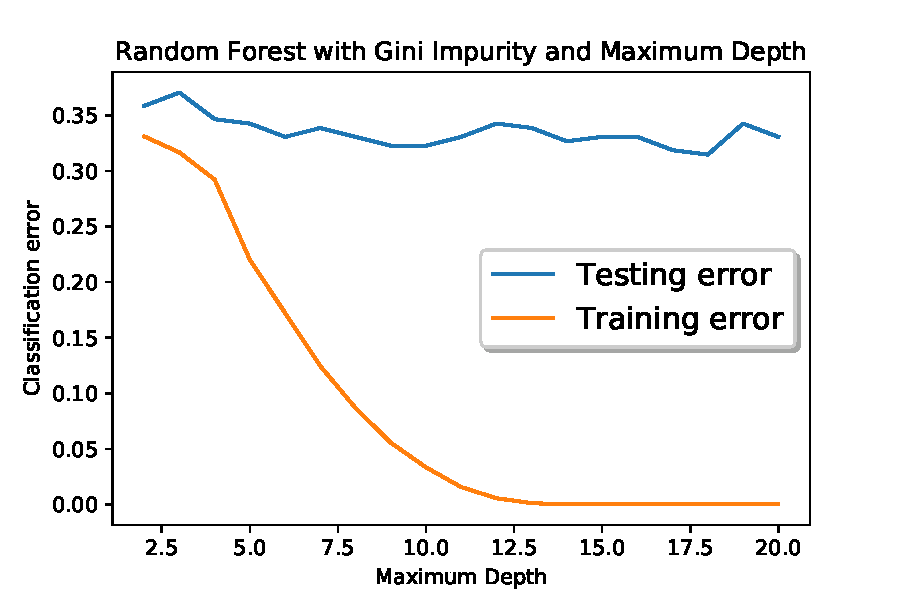
\includegraphics[width=0.49\textwidth]{RT_max_depth.pdf}}
      \end{figure}
\end{solution}

\problem\textbf{[2 points, Extra Credit] }For the stopping criterion tested in \textbf{Problem F}, which parameter value minimizes the decision tree and random forest test error respectively? 

\begin{solution}
   The error is minimised at a max depth of 2 and 18, respectively.
\end{solution}



\newpage
\section{The AdaBoost Algorithm [40 points]}
\materials{Lecture 6}

In this problem, you will show that the choice of the $\alpha_t$ parameter in
the AdaBoost algorithm corresponds to greedily minimizing an exponential upper
bound on the loss term at each iteration.

\problem[3]
Let $h_t: \mathbb{R}^m \rightarrow \{-1,1\}$ be the weak classifier obtained at step $t$, and let $\alpha_t$ be
its weight. Recall that the final classifier is $$H(x) = \text{sign}(f(x)) = \text{sign} \left(\sum\limits_{i=1}^T \alpha_{t}h_t(x) \right).$$

Suppose $\{(x_1, y_1), ..., (x_N, y_N)\} \subset \mathbb{R}^m \times \{-1,1\}$ is our training dataset.  Show that the training set error of the final classifier can be bounded from
above if an an exponential loss function is used:

$$E = \frac{1}{N} \sum\limits_{i=1}^N \exp(-y_{i}f(x_i)) \geq \frac{1}{N} \sum\limits_{i=1}^N \mathbbm{1}(H(x_i) \neq y_i),$$

where $\mathbbm{1}$ is the indicator function.

\begin{solution}
 Given all terms in the above sums are positive, all we need to prove is:
 \begin{equation}
     \exp{(-y_if(x_i))}\geq \mathbbm{1}(H(x_i)\neq y_i)
 \end{equation}
 For the case where $y_i$ and $f(x_i)$ have different signs, we have:
 \begin{equation}
    \exp{(-y_if(x_i))}\geq 1
 \end{equation}
 and:
 \begin{equation}
    \mathbbm{1}(H(x_i)\neq y_i)=1
 \end{equation}
 Similarly, for $y_i$ and $f(x_i)$ being the same sign, we have:
 \begin{equation}
    \exp{(-y_if(x_i))}\geq 0
 \end{equation}
 and:
 \begin{equation}
    \mathbbm{1}(H(x_i)\neq y_i)=0
 \end{equation}
 As such, we find:
 \begin{equation}
    \exp{(-y_if(x_i))}\geq \mathbbm{1}(H(x_i)\neq y_i)
 \end{equation}
 meaning:
 \begin{equation}
    E = \frac{1}{N} \sum\limits_{i=1}^N \exp(-y_{i}f(x_i)) \geq \frac{1}{N} \sum\limits_{i=1}^N \mathbbm{1}(H(x_i) \neq y_i)
 \end{equation}
\end{solution}

\problem[3]
Find $D_{T + 1}(i)$ in terms of $Z_t$, $\alpha_t$, $x_i$, $y_i$, and the classifier $h_t$, where $T$ is the last timestep and $t \in \{1, \ldots, T\}$. Recall that $Z_t$ is the normalization factor for distribution $D_{t+1}$:
$$Z_t = \sum\limits_{i=1}^N D_t(i) \exp(-\alpha_{t}y_{i}h_{t}(x_{i})).$$

\begin{solution}
 From lectures, we know:
 \begin{equation}
     D_{t+1}(i) = \frac{D_t(i)\exp{(-\alpha_ty_ih_t(x_i))}}{Z_t}
 \end{equation}
 This is a recursive relationship which, when fully expanded, gives:
 \begin{equation}
    D_{t}(i) =D_1(i)\prod_j^{t-1}\frac{\exp{(-\alpha_jy_ih_j(x_i))}}{Z_j}
\end{equation}
Thus:
\begin{equation}
    D_{T+1}(i) =D_1(i)\prod_j^{T-1}\frac{\exp{(-\alpha_jy_ih_j(x_i))}}{Z_j}
\end{equation}
Substituting $D_1(i)=\frac{1}{T}$ gives:
\begin{equation}
    D_{T+1}(i) =\frac{\prod_j^{T-1}\frac{\exp{(-\alpha_jy_ih_j(x_i))}}{Z_j}}{T}
\end{equation}
\end{solution}

\problem[2]
Show that $E = \sum_{i=1}^N  \frac{1}{N} e^{\sum_{t=1}^T -\alpha_t y_i h_t(x_i)}.$

\begin{solution}
 Given that:
 \begin{equation}
     f(x_i) = \sum_j\alpha_jh_j(x_i)
 \end{equation}
 we obtain:
 \begin{equation}
    E = \sum_{i=1}^N  \frac{1}{N} e^{\sum_{t=1}^T -\alpha_t y_i h_t(x_i)}
 \end{equation}

\end{solution}

\problem[5]
Show that
$$E = \prod\limits_{t=1}^T Z_t.$$

\begin{hint}
	Recall that $\sum_{i = 1}^N D_t(i) = 1$ because $D$ is a distribution.
\end{hint}

\begin{solution}
    Substituting our definition of $D_t(i)$ into our expression for $Z_t$ gives:
    \begin{equation}
        Z_t = \frac{1}{T}\sum\limits_{i=1}^N \left(\prod_j^{t-1}\frac{\exp{(-\alpha_jy_ih_j(x_i))}}{Z_j}\right)\exp(-\alpha_{t}y_{i}h_{t}(x_{i}))
    \end{equation}
    \begin{equation}
        Z_t = \frac{1}{T}\sum\limits_{i=1}^N \left(\prod_j^{t-1}\frac{1}{Z_j}\right)\left(\prod_j^{t}\exp{(-\alpha_jy_ih_j(x_i))}\right)
    \end{equation}
    \begin{equation}
        Z_t = \frac{1}{T}\sum\limits_{i=1}^N \left(\prod_j^{t-1}\frac{1}{Z_j}\right)\exp{\sum_j^t\left(-\alpha_jy_ih_j(x_i)\right)}
    \end{equation}
    Thus:
    \begin{equation}
        \prod_j^{t}Z_j=\frac{1}{T}\sum\limits_{i=1}^N\exp{\sum_j^t\left(-\alpha_jy_ih_j(x_i)\right)}
    \end{equation}
    As we can see, we have:
    \begin{equation}
        E = \prod_j^{T}Z_j
    \end{equation}
\end{solution}

\problem[5]
Show that the normalizer $Z_t$ can be written as
\[Z_t = (1 - \epsilon_t) \exp(-\alpha_t) + \epsilon_{t} \exp(\alpha_t)\]
where $\epsilon_t$ is the training set error of weak classifier $h_t$ for the weighted dataset:
\[\epsilon_t = \sum\limits_{i=1}^N D_t(i)\mathbbm1(h_t(x_i) \neq y_i).\]

\begin{solution}
	Starting from:
    \begin{equation}
        Z_t = \sum\limits_{i=1}^N D_t(i) \exp(-\alpha_{t}y_{i}h_{t}(x_{i}))
    \end{equation}
    Taking the case where $h_t(x_i)\neq y_i$, we have:
    \begin{equation}
        Z_t = \sum\limits_{i=1}^N D_t(i) \exp(\alpha_{t})
    \end{equation}
    By the nature of distribution functions, this gives:
    \begin{equation}
        Z_t = \exp(\alpha_{t})
    \end{equation}
    From the definition of $\epsilon_t$, if $h_t(x_i)\neq y_i$, we have:
    \begin{equation}
        \epsilon_t = \sum\limits_{i=1}^N D_t(i) = 1
    \end{equation}
    Thus:
    \begin{equation}
        Z_t = (0)\exp(-\alpha_t)+\exp(\alpha_t)=\exp(\alpha_t)
    \end{equation}
    Inversly, for $h_t(x_i)= y_i$, we have:
    \begin{equation}
        Z_t = \sum\limits_{i=1}^N D_t(i) \exp(-\alpha_{t})=\exp(-\alpha_{t})
    \end{equation}
    And, given $\epsilon_t=0$:
    \begin{equation}
        Z_t = \exp(-\alpha_t)+(0)\exp(\alpha_t)=\exp(-\alpha_t)
    \end{equation}
    Thus, both cases are satisfied.
\end{solution}

\problem[2]
We derived all of this because it is hard to directly minimize the training set error, but we can greedily minimize the upper bound $E$ on this error. Show that choosing $\alpha_t$
greedily to minimize $Z_t$ at each iteration leads to the choices in
AdaBoost:
$$\alpha_{t}^* = \frac{1}{2} \ln \left(\frac{1 - \epsilon_t}{\epsilon_t} \right).$$

\begin{solution}
	Taking the derivative w.r.t. $\alpha_t$ gives:
    \begin{equation}
        \frac{\partial Z_t}{\partial\alpha_t} = -(1-\epsilon_t)\exp(-\alpha_t)+\epsilon_t\exp(\alpha_t) = 0
    \end{equation}
    \begin{equation}
        \frac{(1-\epsilon_t)}{\epsilon_t} = \exp(2\alpha_t)
    \end{equation}
    \begin{equation}
        \alpha_t^* = \frac{1}{2}\ln \left(\frac{1 - \epsilon_t}{\epsilon_t} \right)
    \end{equation}
\end{solution}

\begin{problem}[14]
    Implement the \texttt{GradientBoosting.fit()} and \texttt{AdaBoost.fit()} methods in the notebook provided for you. Some important notes and guidelines follow:
    \begin{itemize}
        \item For both methods, make sure to work with the class attributes provided to you. Namely, after \texttt{GradientBoosting.fit()} is called, \texttt{self.clfs} should be appropriately filled with the \texttt{self.n_clfs} trained weak hypotheses. Similarly, after \texttt{AdaBoost.fit()} is called, \texttt{self.clfs} and \texttt{self.coefs} should be appropriately filled with the \texttt{self.n_clfs} trained weak hypotheses and their coefficients, respectively.
        \item \texttt{AdaBoost.fit()} should additionally return an $(N, T)$ shaped numpy array \texttt{D} such that \texttt{D[:, t]} contains $D_{t+1}$ for each $t \in \{0, \ldots, \texttt{self.n_clfs}\}$.
        \item For the \texttt{AdaBoost.fit()} method, \textbf{use the 0/1 loss} instead of the exponential loss.
	\item The only Sklearn classes that you may use in implementing your boosting fit functions are the DecisionTreeRegressor and DecisionTreeClassifier, not GradientBoostingRegressor.
    \end{itemize}
\end{problem}

\begin{solution}
  The following figures were generated:
  \begin{itemize}
      \item For Gradient Boost:
      \begin{figure}[H]
        \begin{center}
        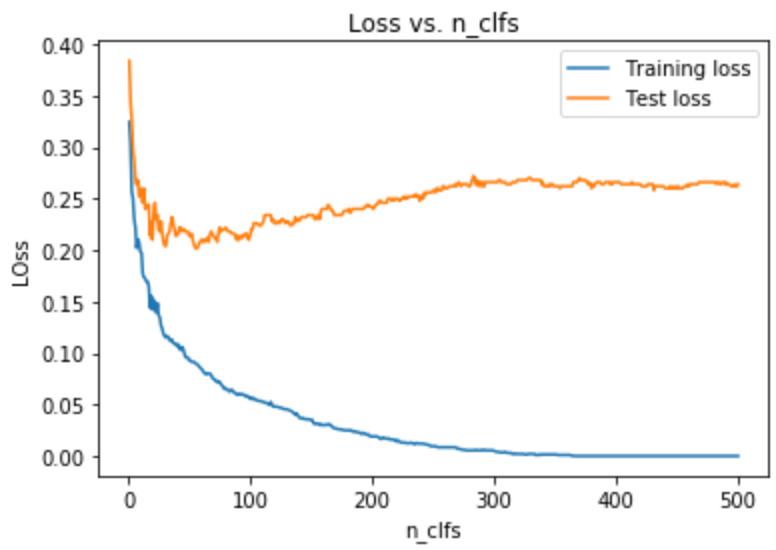
\includegraphics[width=0.5\textwidth]{Loss_GB.png}
        \end{center}
        \end{figure}
      \item For Adaboost:
      \begin{figure}[H]
        \begin{center}
        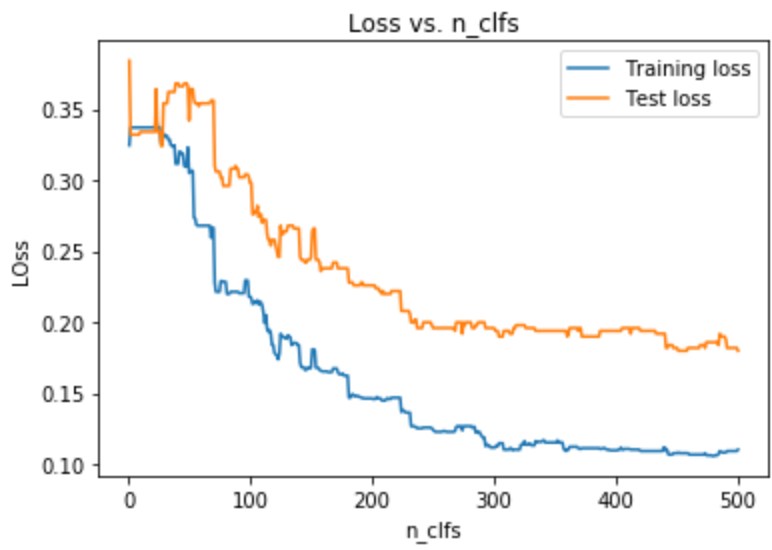
\includegraphics[width=0.5\textwidth]{Loss_AB.png}
        \end{center}
        \end{figure}
  \end{itemize}
\end{solution}

\begin{problem}[2]
    Describe and explain the behaviour of the loss curves for gradient boosting and for AdaBoost. You should consider two kinds of behaviours: the smoothness of the curves and the final values that the curves approach.
\end{problem}

\begin{solution}
  In terms of smoothness, gradient boost is smoother than adaboost; this is primarily because the adaboost method will be jumping between weights as we correctly or incorrectly classify data points, primarily through the definition of our loss function. In gradient boosting, all equations are continuous, resulting in a smooth loss.
  
  In terms of final errors, because gradient boosting is weighing all datapoints equally, it eventually reaches an error of 0. However, in the case of adaboosting, because we are not fitting all the points equally, the error is non-zero even for large numbers of classifiers. However, the testing error for gradient boosting is greater than adaboosting, highlighting that the former is overfitting, primarily because it is fitting all data points equally. 
\end{solution}

\begin{problem}[2]
    Compare the final loss values of the two models. Which performed better on the classification dataset?
\end{problem}

\begin{solution}
  In terms of classification, Adaboost performed better. We can see they by considering that, not only was the final loss smaller than gradient boosting, but, in comparison to the training loss, adaboost had a smaller difference, indicative of a smaller bias, implying that the model generated will generalise better.
\end{solution}

\begin{problem}[2]
    For AdaBoost, where are the dataset weights the largest, and where are they the smallest?
\end{problem}
\begin{hint}
    Watch how the dataset weights change across time in the animation.
\end{hint}
\begin{solution}
   The data points in the center of the spiral have the smallest weights, primarily because they are already fitted correctly, whilst the points at the borders of the spirals have the largest weights, given these are the points we are most focused on fitting.
\end{solution}

\end{document}